\documentclass{article}

\usepackage[utf8]{inputenc} %For non-ASCII characters
\usepackage[a4paper, total={6in, 8in}]{geometry}
\usepackage{listings}
\usepackage{graphicx}
\usepackage{listings} %For code blocks
\usepackage{hyperref} %For URL links
\usepackage{xcolor} %for coloring text
%Bibliography
%\usepackage{biblatex}
\usepackage[backend=biber,style=numeric,sorting=ynt]{biblatex}
\addbibresource{bibliography.bib}


\setlength{\parindent}{0pt} %no indentation

\begin{document}
\begin{minipage}{\textwidth}
  \Large
  \centering
  {\large 34322 Communication Network for Control and Data Acquisition\\}
  Mini-project\\
  LoRa in racing cars\\
  Anders Vedel Eriksen s194017\\
  Date: \today
  \vspace{1cm}
\end{minipage}

\section*{Abstract}
This project concerns the implementation of wireless telemetry for use in student projects such as the Vermilion Racing Team race car at DTU. LoRa and LoRaWAN are introduced and compared with LTE technology, and finally an experiment with a peer-to-peer setup with two LoRa nodes communicating is set up and put to the test. The conclusion on the experiment is that while data can be transferred with high integrity, the transmission time in conjunction with regulations in the EU concerning the duty cycle might make the data rate too slow to use for a live data feel, monitoring sensor data from the car. Further experimentation could be done to better decide if LoRa is a suitable technology for this usecase.

\section{Introduction}
At DTU, several student teams are working with building cars for different purposes. For example, the Ecocar is competing for driving the furthest possible on a liter of fuel, the Solar car is trying to drive on sunpower only, and Vermilion Racing is building an electric racecar to compete in Formula Student. The Vermilion racecar is the inspiration for this project, where the topic is to investigate if LoRa is a suitable technology for wireless telemetry in situations, reading sensors on a high speed moving vehicle in real time.

A concrete case is that the car in the summer is shipped to Italy, where the car is gonna race on the Riccardo Paletti di Varano `de Melegrari racetrack, near Parma. On the track, the distance between the car and the paddock where the team are during the race, is approximately 600 meters, and the biggest distance from one point to another on the track is just shy of one kilometer. The terrain on and around the track is mostly unobstructed.

\section{Technology}
In Formula 1, each car is equipped with over 300 sensors, generating 1.1 million datapoints between the racetrack and the pits\cite{DCFrontier}. Through the years, Formula 1 has adopted new technologies and have traditionally been on the forefront of wireless technology. Different proprietary WiFi solutions have been used for telemetry between the cars on the track, and recently, 5G has been adopted to be used for telemetry\cite{FastCompany}. As 5G is still relatively new, we may not have coverage at the track, so it is safer to base this discussion on 4G/LTE.

\subsection{LTE}
LTE has one big advantage over LoRa, in that it has a much higher bitrate at 300 Mbps download and 75 Mbps upload, or even higher with newer LTE technology\cite{MobilePDF}. 

\section{Lora on RN2483A}

When setting up a LoRa P2P connection, some parameters must be tuned and matched between nodes. The highest possible datarate should be spreading factor 7 with a bandwidth of 250KHz\cite{regparam}. Is a transmitter transmitting with a 125KHz bandwidth, a receiver should receive in a matching 125KHz bandwidth. For maximum signal range, the power of the transmitter should be maximized. The RN2483A is designed to transceive at a power up to 14 dBm. LoRa has some amount of forward error correction built in which can be configured. In an area with high interference, one might choose a high ratio of error correction, while in an area with low interference, a low ratio might be better suited. A high coding rate ratio will make the transmission more reliable, but at the cost of transfer rate\cite{understandingparams}.
\begin{lstlisting}
  loraSerial.println("radio set freq 869100000");   #centerfrequency
  loraSerial.println("radio set sf sf7");           #spread factor
  loraSerial.println("radio set bw 125");           #radio bandwidth
  loraSerial.println("radio set rxbw 125");         #receiver bandwidth
  loraSerial.println("radio set pwr 14")            #power
\end{lstlisting}

\section{Experiment and Results}
A experiment was set up, to see LoRa working. The setup was a NodeMCU microcontroller connected to a Microchip\textregistered  RN2483A LoRa module, working as a transmitter. A similar setup with the same microcontroller and RN2483A LoRa board was set up as receiver, and through a USB cable connected to a PC via UART, communication with serial. The PC is running a python script to read and interpret the incoming data and plotting it on a graph.\\

The transmitter has a preloaded array of twenty values, which when plottet on a time axis shows a sinusoidal wave. Also, a value containing time information is also transmitted. All in all, a 4 byte value is to be transmitted, where the least significant byte is the sinewave value, and the remaining are for the time value. To send a message with the RN2483A board, a command containing a specific string and the data, also transmitted as string type, is send from the microcontroller to the LoRa module via a serial connection. For this program, a virtual serial connection is used between microcontroller and LoRa module, as we want to save the physical UART serial communication in the microcontroller for communication between the receiver microcontroller and the PC. The command for transmitting via serial is:

\begin{lstlisting}
loraserial.println("radio rx " + String(message(), HEX));
\end{lstlisting}

``radio rx'' signals that we want to transmit. In my code, the function message() generates the 4 byte value to transmit, which is converted to a string and formatted in HEX. HEX requires the least amount of characters to transmit, why it is used here. As a visual cue, a LED lights up when a transmission is underway.\\

The receiver is continuously listening for messages. When it has received a message, a led lights up. When a message is picked up on the virtual serial connection between LoRa module and microcontroller, it is forwarded to the PC via the built in UART interface.\\

A Python script is handling the data coming in via the serial connection. When printing the incoming value in the Python terminal, it could look something like this:
\begin{lstlisting}
  data = b'radio rx  0812467F\r\r\n'
\end{lstlisting}
The data is coming in as a byte array of size 21. The actual content of the message is the eight bytes formatted in HEX, `0812467F', where the last two digits represent the least significant byte from the original data, the sinusoidal value. This shows an inefficiency in transmitting; The original 4 byte integer data is formatted in HEX (8 digits), which is transferred as character bytes, taking up 8 bytes (one for each digit/character), double the amount of bits than originally required. While the data is formatted in HEX, it is in fact a byte, meaning that it will have the decimal value of the corresponding character in the ASCII table, being something completely different to the actual value. This is fixed with a few lines of python code:
\begin{lstlisting}
  data = data[10:18]        #data is a byte array of 8 bytes
  data_hex = int(data, 16)  #casts an int, formats in base 16 (HEX)
\end{lstlisting}
The value can now be used, for example plottet to continuously monitor the value. This is what has been done in the following test. On two different days, experiments was carried out. Different spread factors was used, and finally the delay between transmissions was decreased. On day one, with spread factor 7 and 2000ms delay, some transmissions were lost, figure \ref{fig:sf7-2000ms}.

\begin{figure}[h!]
  \centering
  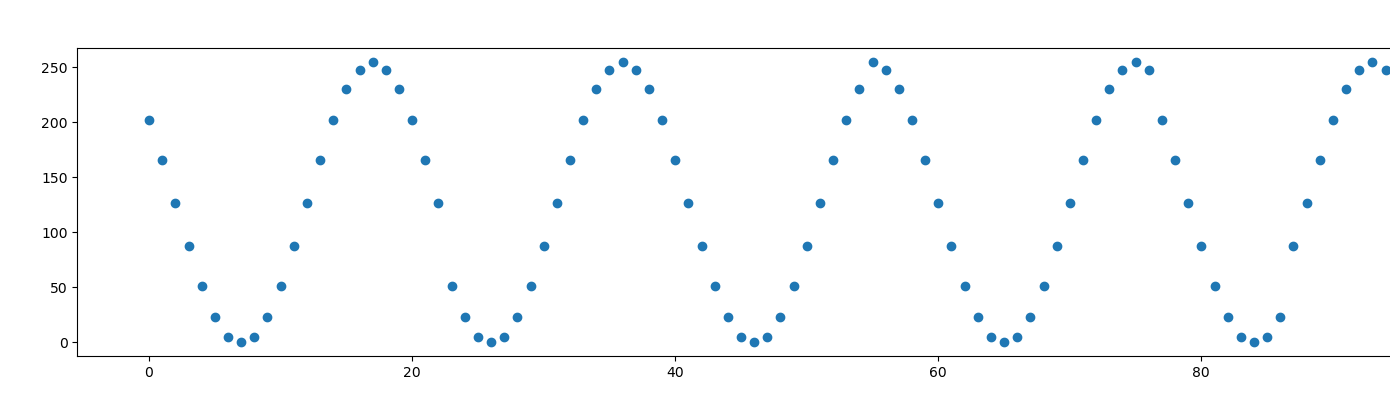
\includegraphics[height = 4cm]{sf7.png}
  \caption{Day 1, sf7, delay 2000 ms}
  \label{fig:sf7-2000ms}
\end{figure}

On the second day, in another building, the same experient was carried out, with no dropped transmissions, figure \ref{fig:sf7-2}.
\begin{figure}[h!]
  \centering
  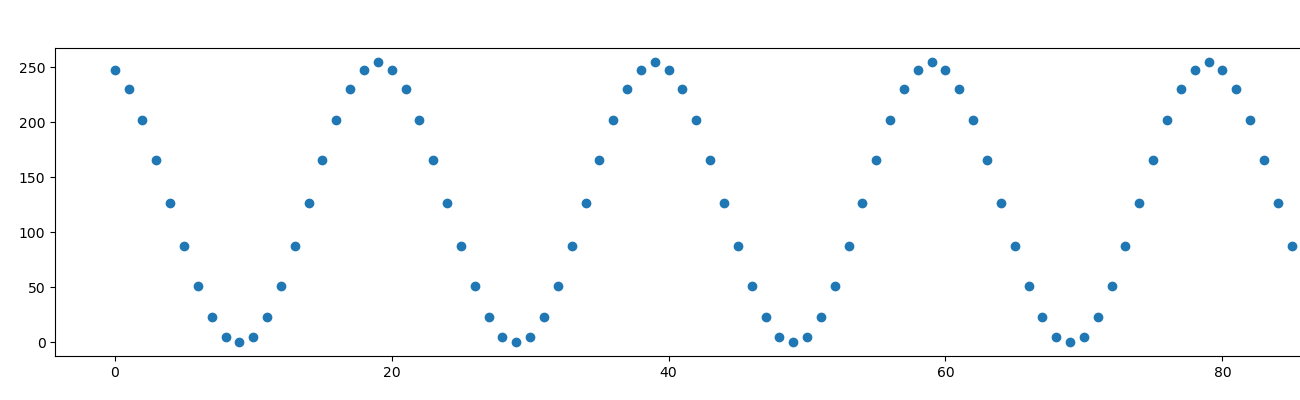
\includegraphics[height = 4cm]{sf7-2.png}
  \caption{Day 2, sf7, delay 2000ms}
  \label{fig:sf7-2}
\end{figure}

To test the datarate, the delay was decreased to 100ms. Furthermore, all unnecesary serial operations was left out to increase microcontroller speed. This resulted in still very few dropped transmissions, see figure \ref{fig:sf7-100ms}. The transmission time was in the microcontroller measured to 20ms.
\begin{figure}[h!]
  \centering
  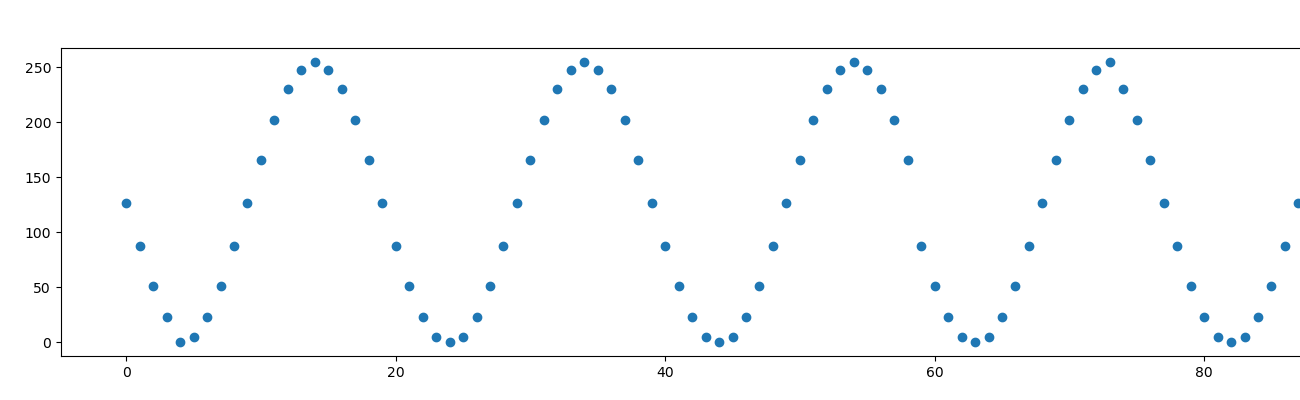
\includegraphics[height = 4cm]{sf7-100ms.png}
  \caption{Day 2, sf7, delay 100 ms}
  \label{fig:sf7-100ms}
\end{figure}
\newpage
On day one, a wider spread factor of 9 was also tested, which worked fine at 2000ms delay, but failed completely at 1000ms delay, figure \ref{fig:sf9}.

\begin{figure}[h!]
  \centering
  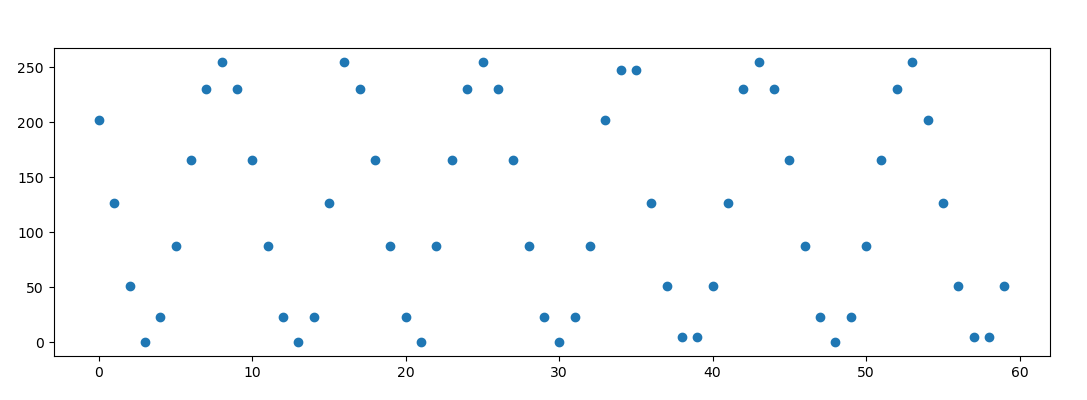
\includegraphics[height = 4cm]{sf91000ms.png}
  \caption{sf9, delay of 1 second}
  \label{fig:sf9}
\end{figure}
\newpage
\subsection*{Conclusion}
There was an obvious difference between the two locations from day one and day two, even though they were both inside buildings, with the same setups and configurations, and in a few instances it seemed the connection was very unreliable. Visual cues showed that transmission seemed two work, but receiving had problems. Maybe the issue was in the microcontroller or the connection between microcontroller and PC, leading to the microcontroller not able to keep up. This could be investigated further. The transmission time could be optimized to 20ms through removing unnecessary serial communication in the transmitter. With the beforementioned duty cycle requirements, this would mean that a transmission could take place every 2000ms, which is slower than what one could wish for in a race situation. Transmission integrity was however very good, with only very few lost transmissions. To really determine if the technology can be used for race cars, the distance between the nodes should be extended to expected real life distance on a race track of approximately 600m, which the transmitter moving at speed. A spread factor of 7 might prove too low here. Experimenting with a 500KHz channel could improve data rate.

\newpage

\section*{Source code}
See files on {\color{red}\href{https://github.com/averiksen/LoRa-mini-projekt}{GitHub}}.

\printbibliography

\end{document}
